\documentclass[1p]{elsarticle_modified}
%\bibliographystyle{elsarticle-num}

%\usepackage[colorlinks]{hyperref}
%\usepackage{abbrmath_seonhwa} %\Abb, \Ascr, \Acal ,\Abf, \Afrak
\usepackage{amsfonts}
\usepackage{amssymb}
\usepackage{amsmath}
\usepackage{amsthm}
\usepackage{scalefnt}
\usepackage{amsbsy}
\usepackage{kotex}
\usepackage{caption}
\usepackage{subfig}
\usepackage{color}
\usepackage{graphicx}
\usepackage{xcolor} %% white, black, red, green, blue, cyan, magenta, yellow
\usepackage{float}
\usepackage{setspace}
\usepackage{hyperref}

\usepackage{tikz}
\usetikzlibrary{arrows}

\usepackage{multirow}
\usepackage{array} % fixed length table
\usepackage{hhline}

%%%%%%%%%%%%%%%%%%%%%
\makeatletter
\renewcommand*\env@matrix[1][\arraystretch]{%
	\edef\arraystretch{#1}%
	\hskip -\arraycolsep
	\let\@ifnextchar\new@ifnextchar
	\array{*\c@MaxMatrixCols c}}
\makeatother %https://tex.stackexchange.com/questions/14071/how-can-i-increase-the-line-spacing-in-a-matrix
%%%%%%%%%%%%%%%

\usepackage[normalem]{ulem}

\newcommand{\msout}[1]{\ifmmode\text{\sout{\ensuremath{#1}}}\else\sout{#1}\fi}
%SOURCE: \msout is \stkout macro in https://tex.stackexchange.com/questions/20609/strikeout-in-math-mode

\newcommand{\cancel}[1]{
	\ifmmode
	{\color{red}\msout{#1}}
	\else
	{\color{red}\sout{#1}}
	\fi
}

\newcommand{\add}[1]{
	{\color{blue}\uwave{#1}}
}

\newcommand{\replace}[2]{
	\ifmmode
	{\color{red}\msout{#1}}{\color{blue}\uwave{#2}}
	\else
	{\color{red}\sout{#1}}{\color{blue}\uwave{#2}}
	\fi
}

\newcommand{\Sol}{\mathcal{S}} %segment
\newcommand{\D}{D} %diagram
\newcommand{\A}{\mathcal{A}} %arc


%%%%%%%%%%%%%%%%%%%%%%%%%%%%%5 test

\def\sl{\operatorname{\textup{SL}}(2,\Cbb)}
\def\psl{\operatorname{\textup{PSL}}(2,\Cbb)}
\def\quan{\mkern 1mu \triangleright \mkern 1mu}

\theoremstyle{definition}
\newtheorem{thm}{Theorem}[section]
\newtheorem{prop}[thm]{Proposition}
\newtheorem{lem}[thm]{Lemma}
\newtheorem{ques}[thm]{Question}
\newtheorem{cor}[thm]{Corollary}
\newtheorem{defn}[thm]{Definition}
\newtheorem{exam}[thm]{Example}
\newtheorem{rmk}[thm]{Remark}
\newtheorem{alg}[thm]{Algorithm}

\newcommand{\I}{\sqrt{-1}}
\begin{document}

%\begin{frontmatter}
%
%\title{Boundary parabolic representations of knots up to 8 crossings}
%
%%% Group authors per affiliation:
%\author{Yunhi Cho} 
%\address{Department of Mathematics, University of Seoul, Seoul, Korea}
%\ead{yhcho@uos.ac.kr}
%
%
%\author{Seonhwa Kim} %\fnref{s_kim}}
%\address{Center for Geometry and Physics, Institute for Basic Science, Pohang, 37673, Korea}
%\ead{ryeona17@ibs.re.kr}
%
%\author{Hyuk Kim}
%\address{Department of Mathematical Sciences, Seoul National University, Seoul 08826, Korea}
%\ead{hyukkim@snu.ac.kr}
%
%\author{Seokbeom Yoon}
%\address{Department of Mathematical Sciences, Seoul National University, Seoul, 08826,  Korea}
%\ead{sbyoon15@snu.ac.kr}
%
%\begin{abstract}
%We find all boundary parabolic representation of knots up to 8 crossings.
%
%\end{abstract}
%\begin{keyword}
%    \MSC[2010] 57M25 
%\end{keyword}
%
%\end{frontmatter}

%\linenumbers
%\tableofcontents
%
\newcommand\colored[1]{\textcolor{white}{\rule[-0.35ex]{0.8em}{1.4ex}}\kern-0.8em\color{red} #1}%
%\newcommand\colored[1]{\textcolor{white}{ #1}\kern-2.17ex	\textcolor{white}{ #1}\kern-1.81ex	\textcolor{white}{ #1}\kern-2.15ex\color{red}#1	}

{\Large $\underline{12a_{0534}~(K12a_{0534})}$}

\setlength{\tabcolsep}{10pt}
\renewcommand{\arraystretch}{1.6}
\vspace{1cm}\begin{tabular}{m{100pt}>{\centering\arraybackslash}m{274pt}}
\multirow{5}{120pt}{
	\centering
	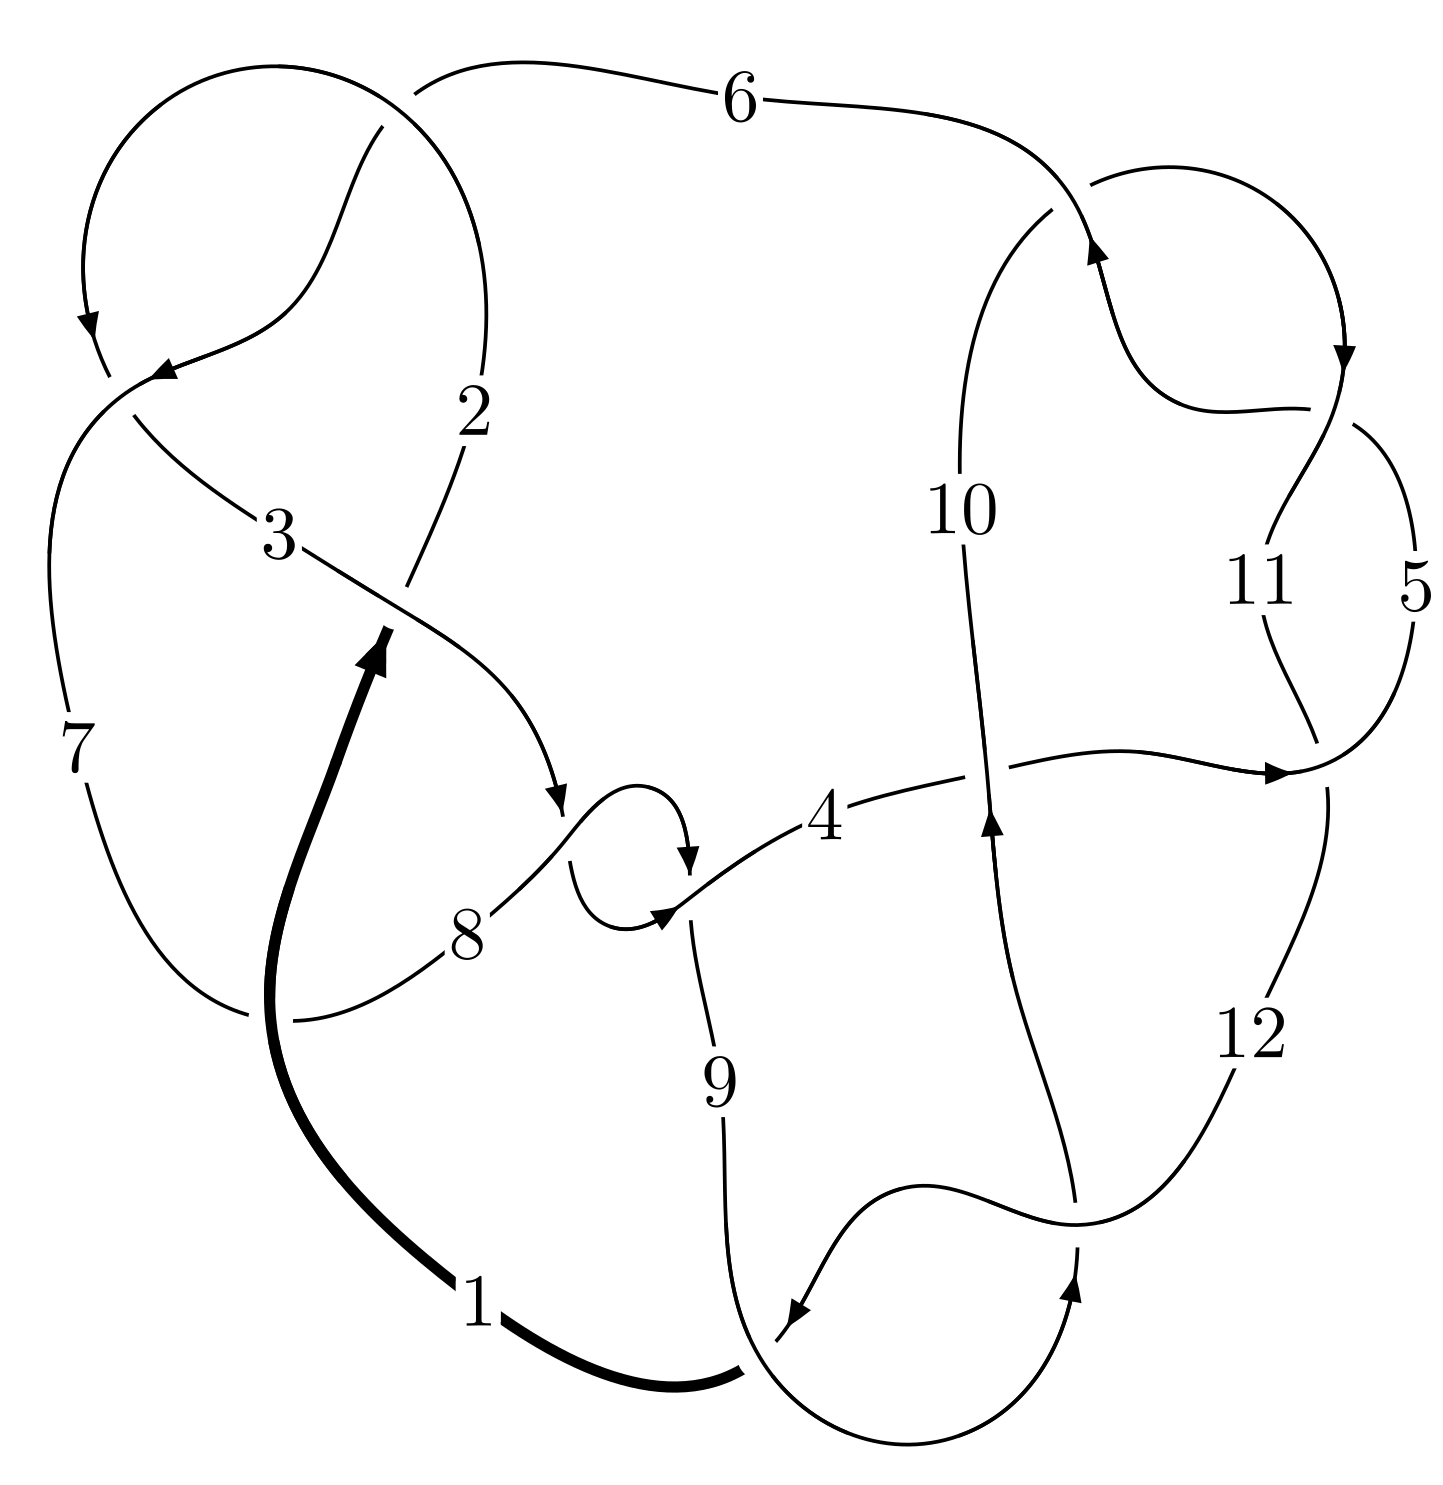
\includegraphics[width=112pt]{../../../GIT/diagram.site/Diagrams/png/1335_12a_0534.png}\\
\ \ \ A knot diagram\footnotemark}&
\allowdisplaybreaks
\textbf{Linearized knot diagam} \\
\cline{2-2}
 &
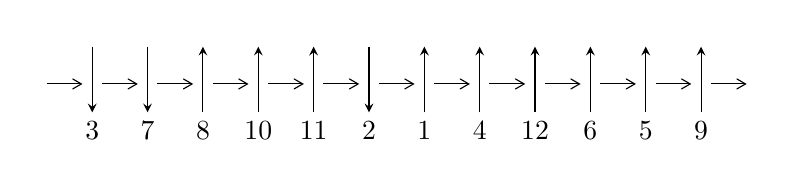
\begin{tikzpicture}[x=20pt, y=17pt]
	% nodes
	\node (C0) at (0, 0) {};
	\node (C1) at (1, 0) {};
	\node (C1U) at (1, +1) {};
	\node (C1D) at (1, -1) {3};

	\node (C2) at (2, 0) {};
	\node (C2U) at (2, +1) {};
	\node (C2D) at (2, -1) {7};

	\node (C3) at (3, 0) {};
	\node (C3U) at (3, +1) {};
	\node (C3D) at (3, -1) {8};

	\node (C4) at (4, 0) {};
	\node (C4U) at (4, +1) {};
	\node (C4D) at (4, -1) {10};

	\node (C5) at (5, 0) {};
	\node (C5U) at (5, +1) {};
	\node (C5D) at (5, -1) {11};

	\node (C6) at (6, 0) {};
	\node (C6U) at (6, +1) {};
	\node (C6D) at (6, -1) {2};

	\node (C7) at (7, 0) {};
	\node (C7U) at (7, +1) {};
	\node (C7D) at (7, -1) {1};

	\node (C8) at (8, 0) {};
	\node (C8U) at (8, +1) {};
	\node (C8D) at (8, -1) {4};

	\node (C9) at (9, 0) {};
	\node (C9U) at (9, +1) {};
	\node (C9D) at (9, -1) {12};

	\node (C10) at (10, 0) {};
	\node (C10U) at (10, +1) {};
	\node (C10D) at (10, -1) {6};

	\node (C11) at (11, 0) {};
	\node (C11U) at (11, +1) {};
	\node (C11D) at (11, -1) {5};

	\node (C12) at (12, 0) {};
	\node (C12U) at (12, +1) {};
	\node (C12D) at (12, -1) {9};
	\node (C13) at (13, 0) {};

	% arrows
	\draw[->,>={angle 60}]
	(C0) edge (C1) (C1) edge (C2) (C2) edge (C3) (C3) edge (C4) (C4) edge (C5) (C5) edge (C6) (C6) edge (C7) (C7) edge (C8) (C8) edge (C9) (C9) edge (C10) (C10) edge (C11) (C11) edge (C12) (C12) edge (C13) ;	\draw[->,>=stealth]
	(C1U) edge (C1D) (C2U) edge (C2D) (C3D) edge (C3U) (C4D) edge (C4U) (C5D) edge (C5U) (C6U) edge (C6D) (C7D) edge (C7U) (C8D) edge (C8U) (C9D) edge (C9U) (C10D) edge (C10U) (C11D) edge (C11U) (C12D) edge (C12U) ;
	\end{tikzpicture} \\
\hhline{~~} \\& 
\textbf{Solving Sequence} \\ \cline{2-2} 
 &
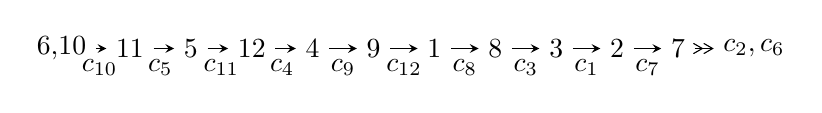
\begin{tikzpicture}[x=22pt, y=7pt]
	% node
	\node (A0) at (-1/8, 0) {6,10};
	\node (A1) at (1, 0) {11};
	\node (A2) at (2, 0) {5};
	\node (A3) at (3, 0) {12};
	\node (A4) at (4, 0) {4};
	\node (A5) at (5, 0) {9};
	\node (A6) at (6, 0) {1};
	\node (A7) at (7, 0) {8};
	\node (A8) at (8, 0) {3};
	\node (A9) at (9, 0) {2};
	\node (A10) at (10, 0) {7};
	\node (C1) at (1/2, -1) {$c_{10}$};
	\node (C2) at (3/2, -1) {$c_{5}$};
	\node (C3) at (5/2, -1) {$c_{11}$};
	\node (C4) at (7/2, -1) {$c_{4}$};
	\node (C5) at (9/2, -1) {$c_{9}$};
	\node (C6) at (11/2, -1) {$c_{12}$};
	\node (C7) at (13/2, -1) {$c_{8}$};
	\node (C8) at (15/2, -1) {$c_{3}$};
	\node (C9) at (17/2, -1) {$c_{1}$};
	\node (C10) at (19/2, -1) {$c_{7}$};
	\node (A11) at (45/4, 0) {$c_{2},c_{6}$};

	% edge
	\draw[->,>=stealth]	
	(A0) edge (A1) (A1) edge (A2) (A2) edge (A3) (A3) edge (A4) (A4) edge (A5) (A5) edge (A6) (A6) edge (A7) (A7) edge (A8) (A8) edge (A9) (A9) edge (A10) ;
	\draw[->>,>={angle 60}]	
	(A10) edge (A11);
\end{tikzpicture} \\ 

\end{tabular} \\

\footnotetext{
The image of knot diagram is generated by the software ``\textbf{Draw programme}" developed by Andrew Bartholomew(\url{http://www.layer8.co.uk/maths/draw/index.htm\#Running-draw}), where we modified some parts for our purpose(\url{https://github.com/CATsTAILs/LinksPainter}).
}\phantom \\ \newline 
\centering \textbf{Ideals for irreducible components\footnotemark of $X_{\text{par}}$} 
 
\begin{align*}
I^u_{1}&=\langle 
u^{81}+u^{80}+\cdots- u-1\rangle \\
\\
\end{align*}
\raggedright * 1 irreducible components of $\dim_{\mathbb{C}}=0$, with total 81 representations.\\
\footnotetext{All coefficients of polynomials are rational numbers. But the coefficients are sometimes approximated in decimal forms when there is not enough margin.}
\newpage
\renewcommand{\arraystretch}{1}
\centering \section*{I. $I^u_{1}= \langle u^{81}+u^{80}+\cdots- u-1 \rangle$}
\flushleft \textbf{(i) Arc colorings}\\
\begin{tabular}{m{7pt} m{180pt} m{7pt} m{180pt} }
\flushright $a_{6}=$&$\begin{pmatrix}0\\u\end{pmatrix}$ \\
\flushright $a_{10}=$&$\begin{pmatrix}1\\0\end{pmatrix}$ \\
\flushright $a_{11}=$&$\begin{pmatrix}1\\- u^2\end{pmatrix}$ \\
\flushright $a_{5}=$&$\begin{pmatrix}- u\\u^3+u\end{pmatrix}$ \\
\flushright $a_{12}=$&$\begin{pmatrix}u^2+1\\- u^4-2 u^2\end{pmatrix}$ \\
\flushright $a_{4}=$&$\begin{pmatrix}- u^3-2 u\\u^3+u\end{pmatrix}$ \\
\flushright $a_{9}=$&$\begin{pmatrix}- u^6-3 u^4-2 u^2+1\\u^8+4 u^6+4 u^4\end{pmatrix}$ \\
\flushright $a_{1}=$&$\begin{pmatrix}u^{10}+5 u^8+8 u^6+3 u^4- u^2+1\\- u^{12}-6 u^{10}-12 u^8-8 u^6- u^4-2 u^2\end{pmatrix}$ \\
\flushright $a_{8}=$&$\begin{pmatrix}- u^{14}-7 u^{12}-18 u^{10}-19 u^8-6 u^6-2 u^4-4 u^2+1\\u^{14}+6 u^{12}+13 u^{10}+12 u^8+6 u^6+4 u^4+u^2\end{pmatrix}$ \\
\flushright $a_{3}=$&$\begin{pmatrix}u^{25}+12 u^{23}+\cdots+4 u^3-3 u\\- u^{25}-11 u^{23}+\cdots-3 u^5+u\end{pmatrix}$ \\
\flushright $a_{2}=$&$\begin{pmatrix}u^{62}+29 u^{60}+\cdots-4 u^2+1\\- u^{62}-28 u^{60}+\cdots-8 u^4- u^2\end{pmatrix}$ \\
\flushright $a_{7}=$&$\begin{pmatrix}u^{36}+17 u^{34}+\cdots-7 u^2+1\\- u^{38}-18 u^{36}+\cdots+10 u^4+u^2\end{pmatrix}$\\&\end{tabular}
\flushleft \textbf{(ii) Obstruction class $= -1$}\\~\\
\flushleft \textbf{(iii) Cusp Shapes $= 4 u^{79}+4 u^{78}+\cdots+16 u+2$}\\~\\
\newpage\renewcommand{\arraystretch}{1}
\flushleft \textbf{(iv) u-Polynomials at the component}\newline \\
\begin{tabular}{m{50pt}|m{274pt}}
Crossings & \hspace{64pt}u-Polynomials at each crossing \\
\hline $$\begin{aligned}c_{1}\end{aligned}$$&$\begin{aligned}
&u^{81}+37 u^{80}+\cdots+5 u+1
\end{aligned}$\\
\hline $$\begin{aligned}c_{2},c_{6}\end{aligned}$$&$\begin{aligned}
&u^{81}- u^{80}+\cdots+u-1
\end{aligned}$\\
\hline $$\begin{aligned}c_{3},c_{8}\end{aligned}$$&$\begin{aligned}
&u^{81}+u^{80}+\cdots-453 u-61
\end{aligned}$\\
\hline $$\begin{aligned}c_{4}\end{aligned}$$&$\begin{aligned}
&u^{81}- u^{80}+\cdots-1961 u-1237
\end{aligned}$\\
\hline $$\begin{aligned}c_{5},c_{10},c_{11}\end{aligned}$$&$\begin{aligned}
&u^{81}+u^{80}+\cdots- u-1
\end{aligned}$\\
\hline $$\begin{aligned}c_{7}\end{aligned}$$&$\begin{aligned}
&u^{81}-3 u^{80}+\cdots+19 u-1
\end{aligned}$\\
\hline $$\begin{aligned}c_{9},c_{12}\end{aligned}$$&$\begin{aligned}
&u^{81}+13 u^{80}+\cdots-5071 u-283
\end{aligned}$\\
\hline
\end{tabular}\\~\\
\newpage\renewcommand{\arraystretch}{1}
\flushleft \textbf{(v) Riley Polynomials at the component}\newline \\
\begin{tabular}{m{50pt}|m{274pt}}
Crossings & \hspace{64pt}Riley Polynomials at each crossing \\
\hline $$\begin{aligned}c_{1}\end{aligned}$$&$\begin{aligned}
&y^{81}+15 y^{80}+\cdots-7 y-1
\end{aligned}$\\
\hline $$\begin{aligned}c_{2},c_{6}\end{aligned}$$&$\begin{aligned}
&y^{81}-37 y^{80}+\cdots+5 y-1
\end{aligned}$\\
\hline $$\begin{aligned}c_{3},c_{8}\end{aligned}$$&$\begin{aligned}
&y^{81}-53 y^{80}+\cdots+186177 y-3721
\end{aligned}$\\
\hline $$\begin{aligned}c_{4}\end{aligned}$$&$\begin{aligned}
&y^{81}+23 y^{80}+\cdots-35110083 y-1530169
\end{aligned}$\\
\hline $$\begin{aligned}c_{5},c_{10},c_{11}\end{aligned}$$&$\begin{aligned}
&y^{81}+75 y^{80}+\cdots+5 y-1
\end{aligned}$\\
\hline $$\begin{aligned}c_{7}\end{aligned}$$&$\begin{aligned}
&y^{81}+7 y^{80}+\cdots+145 y-1
\end{aligned}$\\
\hline $$\begin{aligned}c_{9},c_{12}\end{aligned}$$&$\begin{aligned}
&y^{81}+59 y^{80}+\cdots-6263 y-80089
\end{aligned}$\\
\hline
\end{tabular}\\~\\
\newpage\flushleft \textbf{(vi) Complex Volumes and Cusp Shapes}
$$\begin{array}{c|c|c}  
\text{Solutions to }I^u_{1}& \I (\text{vol} + \sqrt{-1}CS) & \text{Cusp shape}\\
 \hline 
\begin{aligned}
u &= \phantom{-}0.197771 + 1.183570 I\end{aligned}
 & \phantom{-}0.84481 - 3.23672 I & \phantom{-0.000000 } 0 \\ \hline\begin{aligned}
u &= \phantom{-}0.197771 - 1.183570 I\end{aligned}
 & \phantom{-}0.84481 + 3.23672 I & \phantom{-0.000000 } 0 \\ \hline\begin{aligned}
u &= \phantom{-}0.046171 + 1.211660 I\end{aligned}
 & -2.27651 + 1.93915 I & \phantom{-0.000000 } 0 \\ \hline\begin{aligned}
u &= \phantom{-}0.046171 - 1.211660 I\end{aligned}
 & -2.27651 - 1.93915 I & \phantom{-0.000000 } 0 \\ \hline\begin{aligned}
u &= -0.204035 + 1.199890 I\end{aligned}
 & \phantom{-}2.50774 - 1.86243 I & \phantom{-0.000000 } 0 \\ \hline\begin{aligned}
u &= -0.204035 - 1.199890 I\end{aligned}
 & \phantom{-}2.50774 + 1.86243 I & \phantom{-0.000000 } 0 \\ \hline\begin{aligned}
u &= -0.688192 + 0.370410 I\end{aligned}
 & -0.29265 - 12.11820 I & \phantom{-}5.45285 + 10.14700 I \\ \hline\begin{aligned}
u &= -0.688192 - 0.370410 I\end{aligned}
 & -0.29265 + 12.11820 I & \phantom{-}5.45285 - 10.14700 I \\ \hline\begin{aligned}
u &= \phantom{-}0.682734 + 0.364569 I\end{aligned}
 & \phantom{-}1.77767 + 6.96994 I & \phantom{-}8.59265 - 6.07951 I \\ \hline\begin{aligned}
u &= \phantom{-}0.682734 - 0.364569 I\end{aligned}
 & \phantom{-}1.77767 - 6.96994 I & \phantom{-}8.59265 + 6.07951 I \\ \hline\begin{aligned}
u &= -0.667182 + 0.376841 I\end{aligned}
 & -3.10444 - 4.74353 I & \phantom{-}1.89111 + 5.31075 I \\ \hline\begin{aligned}
u &= -0.667182 - 0.376841 I\end{aligned}
 & -3.10444 + 4.74353 I & \phantom{-}1.89111 - 5.31075 I \\ \hline\begin{aligned}
u &= \phantom{-}0.627167 + 0.427079 I\end{aligned}
 & -5.80126 + 5.75467 I & -0.15516 - 7.51536 I \\ \hline\begin{aligned}
u &= \phantom{-}0.627167 - 0.427079 I\end{aligned}
 & -5.80126 - 5.75467 I & -0.15516 + 7.51536 I \\ \hline\begin{aligned}
u &= \phantom{-}0.669087 + 0.343377 I\end{aligned}
 & \phantom{-}2.54734 + 4.35898 I & \phantom{-}9.79953 - 6.09005 I \\ \hline\begin{aligned}
u &= \phantom{-}0.669087 - 0.343377 I\end{aligned}
 & \phantom{-}2.54734 - 4.35898 I & \phantom{-}9.79953 + 6.09005 I \\ \hline\begin{aligned}
u &= -0.220135 + 1.228700 I\end{aligned}
 & \phantom{-}2.26970 - 4.55930 I & \phantom{-0.000000 } 0 \\ \hline\begin{aligned}
u &= -0.220135 - 1.228700 I\end{aligned}
 & \phantom{-}2.26970 + 4.55930 I & \phantom{-0.000000 } 0 \\ \hline\begin{aligned}
u &= \phantom{-}0.600027 + 0.450919 I\end{aligned}
 & -5.90992 - 1.73415 I & -0.700518 + 0.546897 I \\ \hline\begin{aligned}
u &= \phantom{-}0.600027 - 0.450919 I\end{aligned}
 & -5.90992 + 1.73415 I & -0.700518 - 0.546897 I \\ \hline\begin{aligned}
u &= -0.518361 + 0.541766 I\end{aligned}
 & -0.99512 + 8.05238 I & \phantom{-}3.71543 - 4.26648 I \\ \hline\begin{aligned}
u &= -0.518361 - 0.541766 I\end{aligned}
 & -0.99512 - 8.05238 I & \phantom{-}3.71543 + 4.26648 I \\ \hline\begin{aligned}
u &= \phantom{-}0.186058 + 1.245240 I\end{aligned}
 & -2.71415 + 2.87763 I & \phantom{-0.000000 } 0 \\ \hline\begin{aligned}
u &= \phantom{-}0.186058 - 1.245240 I\end{aligned}
 & -2.71415 - 2.87763 I & \phantom{-0.000000 } 0 \\ \hline\begin{aligned}
u &= \phantom{-}0.227678 + 1.238350 I\end{aligned}
 & \phantom{-}0.40246 + 9.70206 I & \phantom{-0.000000 } 0 \\ \hline\begin{aligned}
u &= \phantom{-}0.227678 - 1.238350 I\end{aligned}
 & \phantom{-}0.40246 - 9.70206 I & \phantom{-0.000000 } 0 \\ \hline\begin{aligned}
u &= -0.661462 + 0.328497 I\end{aligned}
 & \phantom{-}1.155840 + 0.658240 I & \phantom{-}7.68128 + 0.74467 I \\ \hline\begin{aligned}
u &= -0.661462 - 0.328497 I\end{aligned}
 & \phantom{-}1.155840 - 0.658240 I & \phantom{-}7.68128 - 0.74467 I \\ \hline\begin{aligned}
u &= \phantom{-}0.504244 + 0.533281 I\end{aligned}
 & \phantom{-}1.06272 - 2.96937 I & \phantom{-}6.86213 + 0.09191 I \\ \hline\begin{aligned}
u &= \phantom{-}0.504244 - 0.533281 I\end{aligned}
 & \phantom{-}1.06272 + 2.96937 I & \phantom{-}6.86213 - 0.09191 I\\
 \hline 
 \end{array}$$\newpage$$\begin{array}{c|c|c}  
\text{Solutions to }I^u_{1}& \I (\text{vol} + \sqrt{-1}CS) & \text{Cusp shape}\\
 \hline 
\begin{aligned}
u &= -0.599806 + 0.419570 I\end{aligned}
 & -2.86954 - 1.93751 I & \phantom{-}3.68977 + 3.76519 I \\ \hline\begin{aligned}
u &= -0.599806 - 0.419570 I\end{aligned}
 & -2.86954 + 1.93751 I & \phantom{-}3.68977 - 3.76519 I \\ \hline\begin{aligned}
u &= -0.528049 + 0.500416 I\end{aligned}
 & -3.65675 + 0.77452 I & \phantom{-}0.180179 + 1.063801 I \\ \hline\begin{aligned}
u &= -0.528049 - 0.500416 I\end{aligned}
 & -3.65675 - 0.77452 I & \phantom{-}0.180179 - 1.063801 I \\ \hline\begin{aligned}
u &= \phantom{-}0.445960 + 0.514360 I\end{aligned}
 & \phantom{-}1.74475 - 0.56616 I & \phantom{-}7.81141 - 0.32467 I \\ \hline\begin{aligned}
u &= \phantom{-}0.445960 - 0.514360 I\end{aligned}
 & \phantom{-}1.74475 + 0.56616 I & \phantom{-}7.81141 + 0.32467 I \\ \hline\begin{aligned}
u &= \phantom{-}0.090833 + 1.321820 I\end{aligned}
 & -3.48103 + 1.92013 I & \phantom{-0.000000 } 0 \\ \hline\begin{aligned}
u &= \phantom{-}0.090833 - 1.321820 I\end{aligned}
 & -3.48103 - 1.92013 I & \phantom{-0.000000 } 0 \\ \hline\begin{aligned}
u &= \phantom{-}0.664571 + 0.032433 I\end{aligned}
 & \phantom{-}4.28824 + 6.44063 I & \phantom{-}11.37631 - 5.73427 I \\ \hline\begin{aligned}
u &= \phantom{-}0.664571 - 0.032433 I\end{aligned}
 & \phantom{-}4.28824 - 6.44063 I & \phantom{-}11.37631 + 5.73427 I \\ \hline\begin{aligned}
u &= -0.660958 + 0.017589 I\end{aligned}
 & \phantom{-}6.06487 - 1.33192 I & \phantom{-}14.4027 + 0.6799 I \\ \hline\begin{aligned}
u &= -0.660958 - 0.017589 I\end{aligned}
 & \phantom{-}6.06487 + 1.33192 I & \phantom{-}14.4027 - 0.6799 I \\ \hline\begin{aligned}
u &= -0.394768 + 0.518007 I\end{aligned}
 & \phantom{-}0.25427 - 4.31628 I & \phantom{-}4.96258 + 5.88678 I \\ \hline\begin{aligned}
u &= -0.394768 - 0.518007 I\end{aligned}
 & \phantom{-}0.25427 + 4.31628 I & \phantom{-}4.96258 - 5.88678 I \\ \hline\begin{aligned}
u &= -0.042555 + 1.365360 I\end{aligned}
 & -6.77977 + 0.65328 I & \phantom{-0.000000 } 0 \\ \hline\begin{aligned}
u &= -0.042555 - 1.365360 I\end{aligned}
 & -6.77977 - 0.65328 I & \phantom{-0.000000 } 0 \\ \hline\begin{aligned}
u &= -0.110213 + 1.375120 I\end{aligned}
 & -5.52185 - 6.10195 I & \phantom{-0.000000 } 0 \\ \hline\begin{aligned}
u &= -0.110213 - 1.375120 I\end{aligned}
 & -5.52185 + 6.10195 I & \phantom{-0.000000 } 0 \\ \hline\begin{aligned}
u &= \phantom{-}0.601777\phantom{ +0.000000I}\end{aligned}
 & \phantom{-}1.08479\phantom{ +0.000000I} & \phantom{-}8.90280\phantom{ +0.000000I} \\ \hline\begin{aligned}
u &= -0.541617 + 0.228507 I\end{aligned}
 & -0.25287 - 3.77283 I & \phantom{-}7.91061 + 8.40043 I \\ \hline\begin{aligned}
u &= -0.541617 - 0.228507 I\end{aligned}
 & -0.25287 + 3.77283 I & \phantom{-}7.91061 - 8.40043 I \\ \hline\begin{aligned}
u &= -0.19013 + 1.41345 I\end{aligned}
 & -5.52475 - 6.36348 I & \phantom{-0.000000 } 0 \\ \hline\begin{aligned}
u &= -0.19013 - 1.41345 I\end{aligned}
 & -5.52475 + 6.36348 I & \phantom{-0.000000 } 0 \\ \hline\begin{aligned}
u &= \phantom{-}0.17372 + 1.43625 I\end{aligned}
 & -4.34343 + 1.67894 I & \phantom{-0.000000 } 0 \\ \hline\begin{aligned}
u &= \phantom{-}0.17372 - 1.43625 I\end{aligned}
 & -4.34343 - 1.67894 I & \phantom{-0.000000 } 0 \\ \hline\begin{aligned}
u &= -0.25166 + 1.43227 I\end{aligned}
 & -4.49351 - 2.67497 I & \phantom{-0.000000 } 0 \\ \hline\begin{aligned}
u &= -0.25166 - 1.43227 I\end{aligned}
 & -4.49351 + 2.67497 I & \phantom{-0.000000 } 0 \\ \hline\begin{aligned}
u &= \phantom{-}0.25453 + 1.43844 I\end{aligned}
 & -3.17261 + 7.73200 I & \phantom{-0.000000 } 0 \\ \hline\begin{aligned}
u &= \phantom{-}0.25453 - 1.43844 I\end{aligned}
 & -3.17261 - 7.73200 I & \phantom{-0.000000 } 0 \\ \hline\begin{aligned}
u &= \phantom{-}0.25853 + 1.44805 I\end{aligned}
 & -4.04746 + 10.40670 I & \phantom{-0.000000 } 0\\
 \hline 
 \end{array}$$\newpage$$\begin{array}{c|c|c}  
\text{Solutions to }I^u_{1}& \I (\text{vol} + \sqrt{-1}CS) & \text{Cusp shape}\\
 \hline 
\begin{aligned}
u &= \phantom{-}0.25853 - 1.44805 I\end{aligned}
 & -4.04746 - 10.40670 I & \phantom{-0.000000 } 0 \\ \hline\begin{aligned}
u &= \phantom{-}0.17326 + 1.46090 I\end{aligned}
 & -5.28963 - 0.54466 I & \phantom{-0.000000 } 0 \\ \hline\begin{aligned}
u &= \phantom{-}0.17326 - 1.46090 I\end{aligned}
 & -5.28963 + 0.54466 I & \phantom{-0.000000 } 0 \\ \hline\begin{aligned}
u &= -0.25138 + 1.45103 I\end{aligned}
 & -8.98223 - 8.10218 I & \phantom{-0.000000 } 0 \\ \hline\begin{aligned}
u &= -0.25138 - 1.45103 I\end{aligned}
 & -8.98223 + 8.10218 I & \phantom{-0.000000 } 0 \\ \hline\begin{aligned}
u &= -0.22226 + 1.45599 I\end{aligned}
 & -8.89843 - 4.95649 I & \phantom{-0.000000 } 0 \\ \hline\begin{aligned}
u &= -0.22226 - 1.45599 I\end{aligned}
 & -8.89843 + 4.95649 I & \phantom{-0.000000 } 0 \\ \hline\begin{aligned}
u &= -0.18698 + 1.46218 I\end{aligned}
 & -9.93180 - 1.82433 I & \phantom{-0.000000 } 0 \\ \hline\begin{aligned}
u &= -0.18698 - 1.46218 I\end{aligned}
 & -9.93180 + 1.82433 I & \phantom{-0.000000 } 0 \\ \hline\begin{aligned}
u &= -0.26014 + 1.45096 I\end{aligned}
 & -6.1479 - 15.5799 I & \phantom{-0.000000 } 0 \\ \hline\begin{aligned}
u &= -0.26014 - 1.45096 I\end{aligned}
 & -6.1479 + 15.5799 I & \phantom{-0.000000 } 0 \\ \hline\begin{aligned}
u &= -0.17307 + 1.46742 I\end{aligned}
 & -7.42202 + 5.58777 I & \phantom{-0.000000 } 0 \\ \hline\begin{aligned}
u &= -0.17307 - 1.46742 I\end{aligned}
 & -7.42202 - 5.58777 I & \phantom{-0.000000 } 0 \\ \hline\begin{aligned}
u &= \phantom{-}0.22921 + 1.46252 I\end{aligned}
 & -11.8872 + 8.8870 I & \phantom{-0.000000 } 0 \\ \hline\begin{aligned}
u &= \phantom{-}0.22921 - 1.46252 I\end{aligned}
 & -11.8872 - 8.8870 I & \phantom{-0.000000 } 0 \\ \hline\begin{aligned}
u &= \phantom{-}0.21649 + 1.46473 I\end{aligned}
 & -12.07490 + 1.25015 I & \phantom{-0.000000 } 0 \\ \hline\begin{aligned}
u &= \phantom{-}0.21649 - 1.46473 I\end{aligned}
 & -12.07490 - 1.25015 I & \phantom{-0.000000 } 0 \\ \hline\begin{aligned}
u &= \phantom{-}0.469947 + 0.071920 I\end{aligned}
 & \phantom{-}0.851920 + 0.071772 I & \phantom{-}12.35395 - 1.18798 I \\ \hline\begin{aligned}
u &= \phantom{-}0.469947 - 0.071920 I\end{aligned}
 & \phantom{-}0.851920 - 0.071772 I & \phantom{-}12.35395 + 1.18798 I \\ \hline\begin{aligned}
u &= -0.145910 + 0.409235 I\end{aligned}
 & -1.47601 + 1.33170 I & \phantom{-}0.709363 - 0.772030 I \\ \hline\begin{aligned}
u &= -0.145910 - 0.409235 I\end{aligned}
 & -1.47601 - 1.33170 I & \phantom{-}0.709363 + 0.772030 I\\
 \hline 
 \end{array}$$\newpage
\newpage\renewcommand{\arraystretch}{1}
\centering \section*{ II. u-Polynomials}
\begin{tabular}{m{50pt}|m{274pt}}
Crossings & \hspace{64pt}u-Polynomials at each crossing \\
\hline $$\begin{aligned}c_{1}\end{aligned}$$&$\begin{aligned}
&u^{81}+37 u^{80}+\cdots+5 u+1
\end{aligned}$\\
\hline $$\begin{aligned}c_{2},c_{6}\end{aligned}$$&$\begin{aligned}
&u^{81}- u^{80}+\cdots+u-1
\end{aligned}$\\
\hline $$\begin{aligned}c_{3},c_{8}\end{aligned}$$&$\begin{aligned}
&u^{81}+u^{80}+\cdots-453 u-61
\end{aligned}$\\
\hline $$\begin{aligned}c_{4}\end{aligned}$$&$\begin{aligned}
&u^{81}- u^{80}+\cdots-1961 u-1237
\end{aligned}$\\
\hline $$\begin{aligned}c_{5},c_{10},c_{11}\end{aligned}$$&$\begin{aligned}
&u^{81}+u^{80}+\cdots- u-1
\end{aligned}$\\
\hline $$\begin{aligned}c_{7}\end{aligned}$$&$\begin{aligned}
&u^{81}-3 u^{80}+\cdots+19 u-1
\end{aligned}$\\
\hline $$\begin{aligned}c_{9},c_{12}\end{aligned}$$&$\begin{aligned}
&u^{81}+13 u^{80}+\cdots-5071 u-283
\end{aligned}$\\
\hline
\end{tabular}\newpage\renewcommand{\arraystretch}{1}
\centering \section*{ III. Riley Polynomials}
\begin{tabular}{m{50pt}|m{274pt}}
Crossings & \hspace{64pt}Riley Polynomials at each crossing \\
\hline $$\begin{aligned}c_{1}\end{aligned}$$&$\begin{aligned}
&y^{81}+15 y^{80}+\cdots-7 y-1
\end{aligned}$\\
\hline $$\begin{aligned}c_{2},c_{6}\end{aligned}$$&$\begin{aligned}
&y^{81}-37 y^{80}+\cdots+5 y-1
\end{aligned}$\\
\hline $$\begin{aligned}c_{3},c_{8}\end{aligned}$$&$\begin{aligned}
&y^{81}-53 y^{80}+\cdots+186177 y-3721
\end{aligned}$\\
\hline $$\begin{aligned}c_{4}\end{aligned}$$&$\begin{aligned}
&y^{81}+23 y^{80}+\cdots-35110083 y-1530169
\end{aligned}$\\
\hline $$\begin{aligned}c_{5},c_{10},c_{11}\end{aligned}$$&$\begin{aligned}
&y^{81}+75 y^{80}+\cdots+5 y-1
\end{aligned}$\\
\hline $$\begin{aligned}c_{7}\end{aligned}$$&$\begin{aligned}
&y^{81}+7 y^{80}+\cdots+145 y-1
\end{aligned}$\\
\hline $$\begin{aligned}c_{9},c_{12}\end{aligned}$$&$\begin{aligned}
&y^{81}+59 y^{80}+\cdots-6263 y-80089
\end{aligned}$\\
\hline
\end{tabular}
\vskip 2pc
\end{document}